\documentclass[11pt]{beamer}
\usetheme{Malmoe}
\usepackage[utf8]{inputenc}
\usepackage[czech]{babel}
\usepackage[T1]{fontenc}
\usepackage{amsmath}
\usepackage{amsfonts}
\usepackage{amssymb}
\usepackage{graphicx}
\usepackage{enumitem}
\usepackage{listings}

% TODO: How to use unicode with listings?
% Jak pouzivat spravne uvozovky?

\author{Jan Tušil}
\title{První kroky s Frama-C}
%\setbeamercovered{transparent} 
%\setbeamertemplate{navigation symbols}{} 
%\logo{} 
%\institute{} 
\date{16. 3. 2015} 
%\subject{} 


\lstset{
	language=C++,
	basicstyle=\ttfamily\footnotesize,
%	keywordstyle=\color{red}
}

% see http://tex.stackexchange.com/questions/130643/nested-itemize-environment-affects-vertical-spacing-of-parent-itemize-environmen
% redefine default beamer item labels
\setitemize{label=\usebeamerfont*{itemize item}%
	  \usebeamercolor[fg]{itemize item}
	    \usebeamertemplate{itemize item}}

\begin{document}

\begin{frame}
\titlepage
\end{frame}

\begin{frame}{Obsah}
\tableofcontents[]
\end{frame}

\section{Úvod}

\begin{frame}{Materiály k prezentaci}
\begin{itemize}
	\item \url{https://github.com/h0nzZik/Frama-C_Examples}
\end{itemize}
\end{frame}

\begin{frame}{Jak získat?}
	\begin{itemize}
		\item Balík frama-c v repozitářích Fedory i Debianu
		\item Alt-Ergo (theorem prover) tamtéž (hodí se pro WP plugin)
	\end{itemize}
\end{frame}

\begin{frame}{Představení}

\begin{figure}
	
\includegraphics[scale=0.3]{frama-c.png}
\end{figure}

\begin{itemize}
	\item<1-> Modulární platforma pro statickou analýzu C kódu
	\item<2-> Jádro
		\begin{itemize}
				\item<4-> Parsování, preprocessing, ,,linkování'' a normalizace kódu
				\item<5-> Ukládání/načítání session
				\item<6-> Uchovávání výsledků práce pluginů
				\item<7-> Manipulace s AST
		\end{itemize}
	\item<3-> Pluginy
		\begin{itemize}
				\item<8-> Analýza závislostí
				\item<9-> Abstraktní interpretace
				\item<10-> Deduktivní verifikace
		\end{itemize}
	\item<11-> Některé pluginy umožňují ověřování programu vůči specifikaci
\end{itemize}

\end{frame}

\begin{frame}{Specifikace?}
	\begin{itemize}
		\item Možné specifikace:
			\begin{itemize}
				\pause \item Za běhu programu nenastane chyba \pause (?)
				\pause \item Chování programu je definované (dle standardu jazyka).
				\pause \item Funkce nemodifikuje globální proměnné
				\pause \item Funkce zachovává vlastnost používané datové struktury
			\end{itemize}
		\pause \item Potřeba jazyka pro zápis specifikace.
	\end{itemize}
\end{frame}


\section{Jazyk ACSL}

\begin{frame}{Jazyk ACSL}

\end{frame}

\subsection{Obecné informace}

\begin{frame}{ACSL - Co je to za jazyk?}
\begin{itemize}
	\item ANSI / ISO C Specification language
	\item Vznikl pro potřeby Frama-C
	\item Vestavěný v komentářích C kódu.
	\item Asserty
	\item Invarianty
	\item Funkční kontrakty (DbC)
	\item http://frama-c.com/acsl.html
\end{itemize}
\end{frame}

\begin{frame}{ACSL - vyjadřovací schopnosti}
\begin{itemize}
	\item C operátory a datové typy
	\item Matematické datové typy
	\item Prvořádová logika (s rozšířeními)
\end{itemize}
\end{frame}


\subsection{Jazykové konstrukce}

\defverbatim[colored]\lstBasicAssert{
\begin{lstlisting}[language=C++]
int x = 17;
/*@ assert x > 5 */
\end{lstlisting}
}

\begin{frame}{Asserty}
\lstBasicAssert
\begin{itemize}
	\item Základní specifikační jednotka
	\item Tvrzení o stavu programu v daném bodě.
	\item (ACSL specifikace zabudována v komentáři)
\end{itemize}
\end{frame}

\defverbatim[colored]\lstQuantifiedAssert{
\begin{lstlisting}
int array[4] = {-15, 3, 17, 104};
/*@
assert \forall integer i, j;
0 <= i <= j < 4 ==> array[i] <= array[j];
*/
\end{lstlisting}
}


\begin{frame}{Kvantifikátory}
\lstQuantifiedAssert
\begin{itemize}
	\item Vázaná proměnná má daný typ
	\item Typ může být uživatelem definovaný (typedef, struct)
	\item \texttt{integer} označuje (matematické) celé číslo
\end{itemize}
\end{frame}


\defverbatim[colored]\lstPointerValidity{
\begin{lstlisting}
int array[4] = {-15, 3, 17, 104};	
/*@ assert \valid(array + (0..3)); */
\end{lstlisting}
}

% TODO: kod na slajdech by mohl byt zarovnany vzdy stejne

\begin{frame}{Pointery}
\lstPointerValidity
\begin{itemize}
	\item Predikát \textbackslash valid bere množinu termů
	\item \(0..3\) označuje množinu \( \{ 0, 1, 2, 3 \} \)
	\item Význam: výrazy \( \{ array + 0, \ldots , array + 3 \} \) jsou platné ukazatele
	\item Obvyklá pointer aritmetika
\end{itemize}
\end{frame}

\defverbatim[colored]\lstPredicateSorted{
\begin{lstlisting}
/*@
predicate is_sorted ( int *array, integer len ) = 
\forall integer i, j; 0 <= i <= j < len
==> array[i] <= array[j];
*/
\end{lstlisting}
}

\defverbatim[colored]\lstPredicateSortedUsed{
\begin{lstlisting}
/*@ assert is_sorted ( array, 4 ); */
\end{lstlisting}
}

\begin{frame}{Uživatelské predikáty}
\lstPredicateSorted
\begin{itemize}
\item Predikát lze využít později
\end{itemize}
\lstPredicateSortedUsed
\end{frame}

\defverbatim[colored]\lstLoopWithInvariant{
\begin{lstlisting}
int arr[7];
[ ... ]
/*@ loop invariant is_sorted(arr, i) */
for ( int i = 0; i < 7; i++ ) {
	[ ... ]
}
\end{lstlisting}
}

\begin{frame}{Invarianty smyček}
\lstLoopWithInvariant
	\begin{itemize}
		\pause \item Invariant musí být platný při (prvním) vstupu do smyčky
		\pause \item Každý průchod smyčkou musí invariant zachovat
	\end{itemize}
\end{frame}

\defverbatim[colored]\lstFunctionContract{
\begin{lstlisting}
/*@
requires \valid ( array + (0 .. ( len-1 ) ) );
ensures is_sorted ( array, len );
assigns \nothing;
 */
void sort ( int *array, size_t len);
\end{lstlisting}
}

\begin{frame}{Funkční kontrakty}
\lstFunctionContract
\begin{itemize}
	\pause \item Co funkce požaduje?
	\pause \item Co funkce garantuje?
	\pause \item Co funkce zachovává / modifikuje?
	\pause \item Paradigma "Design by Contract"
	\pause \item Kde je problém?
\end{itemize}
\end{frame}

\section{Použití Frama-C}

\begin{frame}{Použití Frama-C}

\end{frame}

\begin{frame}{Jednoduché použití}
\begin{itemize}
	\item Soubor hello.c je v adresáři 01\_hello
	\item \lstinline[language=bash]{$ frama-c hello.c -val}
	\pause \item Spustí Value plugin - analýzu možných hodnot proměnných.
	\pause \item Jak ověřit větší projekt z více souborů?
	\pause \item Všechny je vypíšeme na řádce.
\end{itemize}
\end{frame}


\subsection{Příprava zdrojových kódů}

\begin{frame}{Na co je preprocesor v C?}
\begin{itemize}
	\pause \item Makra a náhrady textu
	\pause \item Vkládání (hlavičkových) souborů
\end{itemize}
\end{frame}

\begin{frame}{Preprocessing ve Frama-C}
\begin{itemize}
	\item Výchozí: \lstinline[language=bash]{gcc -C -E -I}
	%FIXME: 'command se zobrazi cervene, protoze je to jeden z builtinu bashe
	\item Možno předefinovat přepínačem \lstinline[language=bash]{\-cpp-command}
	\pause \item Frama-C umí předzpracovat i anotace (s GCC)
	\item Rozpracovaný projekt je možné uložit a znovu načíst
	\item Viz soubor build.mk
\end{itemize}
\end{frame}


\begin{frame}{Drobnosti}
	\begin{itemize}
		\item RTE plugin generuje anotace pro obvyklé runtime chyby
		\item Kombinace RTE + Value může prokázat absenci runtime chyb
		\item Uložený projekt je možné načíst do programu frama-c-gui
	\end{itemize}
\end{frame}

\subsection{Value plugin (+ RTE)}

\begin{frame}{Value plugin}

\end{frame}

\begin{frame}{Value plugin - Principy}
	\begin{itemize}
			\item Abstraktní interpretace
			\item Počítá variační domény proměnných
			\item Overaproximace - dokazuje korektnost
	\end{itemize}
\end{frame}

\begin{frame}{Variační domény}
	\begin{itemize}
			\item Množina možných hodnot, které může obsahovat daná proměnná.
			\item Různé způsoby zápisu
			\begin{itemize}
				\item Výčtem \( \{ 2, 12, 22, 32, 42 \} \)
				\item Intervalem \( [2 \ldots 42], 2 \% 10 \)
			\end{itemize}
	\end{itemize}
\end{frame}

\begin{frame}{Ukázka (01\_hello/hello.c) - 1}
	\begin{figure}
		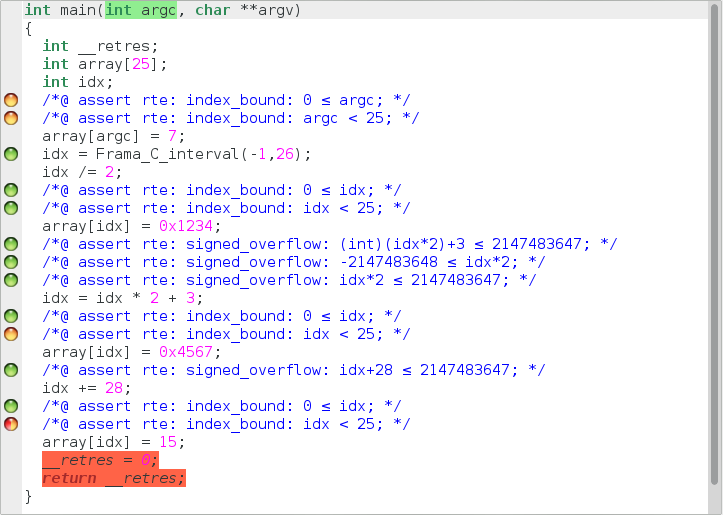
\includegraphics[scale=0.3]{./img/value_01.png}
	\end{figure}
\end{frame}

\defverbatim[colored]\lstFirstValueAnalysis{
\begin{lstlisting}[language=bash]
$ git clone https://github.com/h0nzZik/Frama-C_Examples.git
$ cd Frama-C_Examples/01_hello
$ make
$ frama-c-gui -load project_after_analysis
\end{lstlisting}
}


\begin{frame}{Ukázka (01\_hello/hello.c) - 2}
	\lstFirstValueAnalysis
	\begin{itemize}
			\item Informace vypsané během analýzy jsou k dispozici i v gui
			\item Zajímavé jsou řádky začínající \texttt{hello.c:123:[value]}
			\item Gui zobrazuje variační domény hodnoty proměnných na kartě "Information"
	\end{itemize}
\end{frame}

\defverbatim[colored]\lstFirstValueMainPartOne{
\begin{lstlisting}[language=C++]
int main ( int argc, char *argv[] ) {
/*@ assert rte: index_bound: 0 <= argc; */
/*@ assert rte: index_bound: argc < 25; */
array[argc] = 7;
\end{lstlisting}
}


\begin{frame}{Ukázka (01\_hello/hello.c) - 3}
	\lstFirstValueMainPartOne
\texttt{hello.c:17:[value] Assertion 'rte,index\_bound' got status unknown.}
	\begin{itemize}
			\item Nelze ověřit, že zápis do pole proběhne v pořádku.
			\item Mimochodem, tyto asserty v původním zdrojovém kódu nejsou, byly vygenerovány pluginem RTE. Proto jsou označeny identifikátorem \texttt{rte}.
	\end{itemize}
\end{frame}

\defverbatim[colored]\lstFirstValueMainPartTwo{
\begin{lstlisting}[language=C++]
idx = Frama_C_interval(-1,26);
idx /= 2;
/*@ assert rte: index_bound: 0 < idx; */
/*@ assert rte: index_bound: idx < 25; */
array[idx] = 0x1234;
\end{lstlisting}
}

\begin{frame}{Ukázka (01\_hello/hello.c) - 4}
	\lstFirstValueMainPartTwo
	\texttt{hello.c:20:[value] Assertion 'rte,index\_bound' got status valid.}
	\begin{itemize}
		\item Funkce \texttt{Frama\_C\_interval} vrací nedeterministickou hodnotu ze zadaného intervalu. Je deklarována (i s anotacemi) v souboru \texttt{FRAMA\_C\_SHARE/builtin.h}.
		\item Value plugin spočítá, že po dělení bude proměnná idx ležet v intervalu
			\( [ 0 \ldots 13 ] \)
	\end{itemize}
\end{frame}


\defverbatim[colored]\lstFirstValueMainPartThree{
\begin{lstlisting}{language=C++}
/*@ assert rte: signed_overflow: (int)(idx*2)+3 <= 2147483647; */
/*@ assert rte: signed_overflow: -2147483648 <= idx*2; */
/*@ assert rte: signed_overflow: idx*2 <= 2147483647; */
idx = idx * 2 + 3;
\end{lstlisting}
} % \defverbatim


\begin{frame}{Ukázka (01\_hello/hello.c) - 5}
	\lstFirstValueMainPartThree
	\begin{itemize}
			\item Mnoho lidí neví, že výsledek znaménkového přetečení 
				v jazyce C není definován. RTE plugin to ale ví.
			\item Value určil \( \texttt{idx} \in [3..29],1 \%2 \)

	\end{itemize}
\end{frame}

\defverbatim[colored]\lstFirstValueMainPartFour{
\begin{lstlisting}{language=C++}
/*@ assert rte: index_bound: 0 <= idx; */
/*@ assert rte: index_bound: idx < 25; */
array[idx] = 0x4567;
\end{lstlisting}
} % \defverbatim

\begin{frame}{Ukázka (01\_hello/hello.c) - 6}
	\lstFirstValueMainPartFour

	\begin{itemize}
			\item Value plugin ví, že jistě \( \texttt{idx} \in [3..29],1 \%2 \),
				tedy první assert projde.
			\item Ale protože Value pracuje s overaproximací, nedokáže rozhodnout,
				zda dojde k narušení druhého assertu.
			\item Pokud dojde k runtime chybě, nemá smysl pokračovat v běhu programu.
				Z toho důvodu po provedení uvedeného příkazu Value plugin uvažuje
				pouze hodnoy z intervalu \( [3..23],1\%2 \).
	\end{itemize}
\end{frame}

\defverbatim[colored]\lstFirstValueMainPartFive{
\begin{lstlisting}[language=C++]
idx += 28;
/*@ assert rte: index_bound: 0 <= idx; */
/*@ assert rte: index_bound: idx < 25; */
array[idx] = 15;
\end{lstlisting}
} % \defverbatim

\begin{frame}{Ukázka (01\_hello/hello.c) - 7}
	\lstFirstValueMainPartFive
	\texttt{hello.c:26:[value] Assertion 'rte,index\_bound' got status invalid
	(stopping propagation).}
	\begin{itemize}
		\item Po přičtení bude hodnota proměnné \texttt{idx} větší než 25.
			Assert tedy neprošel.
		\pause \item Kontrola: jaký je zde rozdíl oproti předchozímu případu?
		\pause \item Následující kód je označen za nedosažitelný. Co to znamená v praxi?
	\end{itemize}
\end{frame}

\subsection{WP plugin}

\begin{frame}{WP plugin}

\end{frame}


\begin{frame}{Motivace}
	\begin{itemize}
		\item Value plugin umí dokázat některé vlastnosti funkcí
		\pause \item Některé ale ne.
		\item Vyhodnocování složitých smyček je buď nepřesné
			(odhad invariantu), nebo pomalé (rozbalování).
		\item WP plugin umožňuje dokazovat vlastnosti programů podobně, jako jsme zvyklí dokazovat vlastnosti algoritmů - deduktivně.
		\item Silná podpora Design by Contract
	\end{itemize}
\end{frame}

\defverbatim[colored]\lstExIIwpBash{
\begin{lstlisting}[language=bash]
$ cd Frama-C_Examples/02
$ make
$ frama-c -load frama_project -wp-fct try_initialize_array
\end{lstlisting}
}


\begin{frame}{Ukázkový kód}
	\lstExIIwpBash
	\texttt{[wp] 7 goals scheduled}\\
	\texttt{[wp] [Qed] Goal some\_assert\_1 : Valid} \\
	\texttt{[wp] [Alt-Ergo] Goal some\_assert\_2 : Unknown (Qed:2ms)}
	\begin{itemize}
		\item Soubor \texttt{02/array\_initialization.c}
		\item (Vyplatí se prozkoumat dodané Makefily)
		\item Třeba mít nainstalován theorem prover Alt-Ergo
		\item Možné načíst pomoci \texttt{frama-c-gui}
	\end{itemize}
\end{frame}

\defverbatim[colored]\lstExIIwpItryI{
\begin{lstlisting}[language=C++]
int array[5];
for (int i = 0; i < 5; i++) {
	array[i] = 1 - i;
}
if ( array[2] == -2 )
	array[2]++;
//@ assert array[2] != -2;	
//@ assert array[3] == -2;
\end{lstlisting}
} % \defverbatim

\begin{frame}
	\lstExIIwpItryI
	\begin{itemize}
		\item Toto již jsou ručně psané anotace.
		\item První assert plyne s předchozího IFu.
		\item WP o stavu programu po skončení cyklu nebo volání funkce nepředpokládá vůbec nic. Proto se nepodaří dokázat druhý assert.
		\pause \item Value to zvládne, pokud mu povolíme trávit více času rozbalováním smyček.
	\end{itemize}
\end{frame}

\defverbatim[colored]\lstExIIwpItryII{
\begin{lstlisting}[language=C++]
int array[5];
/*@ loop invariant: \forall integer j;
    0 <= j < i ==> array[j] == 1 - j; */
for (int i = 0; i < 5; i++) {
/*@ assert rte: index_bound: 0 <= i; */
	array[i] = 1 - i;
}
if ( array[2] == -2 )
	array[2]++;
//@ assert array[2] != -2;	
//@ assert array[3] == -2;
\end{lstlisting}
} % \defverbatim

\begin{frame}{S invariantem}
	\lstExIIwpItryII
	\begin{itemize}
			\item Z invariantu lze snadno dokázat požadované vlastnosti.
			\item Invariant ovšem platí pouze za podmínky, že nenastane runtime chyba.
			\item Pokud nelze dokázat RTE assert, invariant nemusí platít.
	\end{itemize}
\end{frame}

\defverbatim[colored]\lstExIIwpItryIII{
\begin{lstlisting}[language=C++]
int array[5];
/*@ loop invariant: \forall integer j;
    0 <= j < i ==> array[j] == 1 - j; */
for (int i = 0; i < 5; i++) {
	i = -1;
/*@ assert rte: index_bound: 0 <= i; */
	array[i] = 1 - i;
}
\end{lstlisting}
} % \defverbatim

\begin{frame}{Podmíněná platnost}
	\lstExIIwpItryIII
	\begin{itemize}
		\item Dojde k runtime chybě (možno zjistit s pomocí Value pluginu)
		\item WP dokáže totéž, co v předchozím případě.
	\end{itemize}
\end{frame}

\defverbatim[colored]\lstExIIwpItryIV{
\begin{lstlisting}[language=C++]
int array[5];
/*@ loop invariant: \forall integer j;
    0 <= j < i ==> array[j] == 1 - j; */
for (int i = 0; i < 5; i++) {
	i = 0;
/*@ assert rte: index_bound: 0 <= i; */
	array[i] = 1 - i;
}
\end{lstlisting}
} % \defverbatim

\begin{frame}{Terminace}
	\lstExIIwpItryIV
	\begin{itemize}
		\item Invariant bezpodmínečně platí (WP ho dokáže)
		\item Tedy asserty také platí
		\pause \item Naneštěstí cyklus neterminuje
	\end{itemize}
\end{frame}

\defverbatim[colored]\lstExIIwpItryV{
\begin{lstlisting}[language=C++]
int array[5];
/*@ loop invariant: 0 <= i <= 5 &&
(   \forall integer j;
0 <= j < i ==> array[j] == 1 - j);
	loop variant 5 - i */
for (int i = 0; i < 5; i++) {
/*@ assert rte: index_bound: 0 <= i; */
	array[i] = 1 - i;
}
\end{lstlisting}
} % \defverbatim

\begin{frame}{Správné řešení}
	\lstExIIwpItryV
	\begin{itemize}
		\item Omezení na proměnnou \texttt{i} vede k platnosti RTE assertu.
		\item Hodnota variantu se snižuje v každém kroku cyklu až k nule.
		\item Program je korektní a terminuje. U rozumných smyček ale není třeba terminaci ověřovat ( a psát varianty)
	\end{itemize}
\end{frame}


\section{Závěr}

\subsection{Výhody}
\begin{frame}{Výhody}
	\begin{itemize}
		\item Široká dokumentace
		\item Snadná instalace
	\end{itemize}
\end{frame}

\subsection{Omezení}

\begin{frame}{Omezení}
\end{frame}

\begin{frame}{Chybějící vlastnosti}
	\begin{itemize}
		\item Pouze C (nepodporuje C++)
		\item Líbilo by se mi:
			\begin{itemize}
				\item Třídy, používání jmenných prostorů (šetří psaní)
			\end{itemize}
		\item Implementována pouze část ACSL
		\item Ošklivé chybové hlášky
	\end{itemize}
\end{frame}


\begin{frame}{Bugy}
	\begin{itemize}
		\item Při výpisu chyb nesedí čísla řádků
		\item Občasný pád grafického rozhraní
	\end{itemize}
\end{frame}



\end{document}
